\chapter{Introduzione}

\section{Ambito del progetto}
BLINC – Blockchain inclusiva per cittadinanze digitali è un progetto di ricerca industriale e sviluppo sperimentale emanato da Regione Piemonte
a valere sui fondi POR FESR 2014-2020 Europei. Il progetto mira a realizzare una piattaforma Blockchain per la gestione di identità digitali,
dati, transazioni di valore coinvolgendo la PA e gli operatori di servizi per i migranti.
Tutti gli attori che entrano in contatto con gli utenti potranno inserire certificazioni:
dal titolo di identità, al credito formativo, alla lettera di raccomandazione che il migrante
potrà esibire a sua discrezione, preservandone la privacy e al contempo migliorando le potenzialità di costruzione di fiducia e inclusione sociale.

La tecnologia blockchain consente di passare da un internet dei dati ad un internet dei valori, promettendo un impatto di innovazione in ambito
finanziario e commerciale paragonabile all’impatto che il web avuto sui modi di comunicare e acquisire informazioni.
La posta in gioco riguarda industrie che generano oltre il 20\% del PIL (stime Wedbush securities). Chiunque sarà in grado di creare coupon,
titoli al portatore sistemi di pagamento, contratti automatici che regolano le relazioni tra diversi attori nella filiera produttiva e molto altro ancora.
Lo sviluppo dell’internet of money è una tendenza già in atto visibile nel successo di strumenti come le gift card, i coupon, i circuiti di credito commerciale,
punti fedeltà, sistemi di pagamento attraverso smartphone.

La blockchain permetterà un salto di qualità rendendo diversi circuiti interoperabili. Si può comprendere la blockchain
in analogia con l’introduzione del protocollo SMTP per la posta elettronica, un’evoluzione dalle intranet aziendali all’internet aperta che conosciamo.
L’ internet delle cose e la diffusione di dispositivi robotici sarà un altro importantissimo driver: operatori come IBM e Samsung prevedono 
he gli oggetti negozieranno tra di loro titoli per l’accesso a dati, energia e rapporti di cooperazione nelle loro funzioni.
Altrettanto significativa è la capacità di sincronizzare le basi dati della pubblica amministrazione, anagrafe, catasto, fisco,
documenti protocollati, ma anche informazioni protette come le registrazioni del sistema sanitario. La proposta presente si inserisce in questo filone di ricerca.

Tutto ciò si integra in un progetto che permette di sperimentare soluzioni originali ad
un problema drammatico, di grande rilevanza politica e sociale, nonché esistenziale.
Essere straniero, provenire da una cultura non europea, talvolta avere una storia di fuga da situazioni insostenibili
o pericolose spesso porta a perdere l’identità formale e sociale costruita nel paese di origine, al tempo stesso la richiesta
di informazione da parte dell’ambiente circostante è maggiore. Dimenticare i propri documenti può causare problemi,
il carico burocratico e la frequenza presso gli uffici della PA sono più alti che per i cittadini italiani.
Attraverso la Blockchain sarà possibile strutturare tecnologie per la fiducia, atte a colmare quel gap di informazione che frena
i processi di inclusione dei migranti, senza portare a stigmatizzazioni o discriminazioni nel diritto alla privacy.

Il funzionamento dell’applicazione base proposta è semplice, un portadocumenti virtuale che contiene certificati auto-generati 
ad esempio a partire da documenti cartacei o per dichiarazione) accanto a documenti generati dei servizi privati e pubblici con cui il migrante viene in contatto.
Il portadocumenti è accessibile da qualsiasi dispositivo, ma pensato per il mobile, con interfacce semplificate che rendono
l’uso compatibile con scarse competenze digitali.

Un altro aspetto fondamentale del prodotto è la gestione granulare della privacy: il portadocumenti non può essere consultato
nella sua interezza, ma, utilizzando tecnologie Blockchain pensate per i record sanitari, l’utente potrà decidere quali certificati ne fanno parte.
L’iniziativa si colloca nel contesto della sharing economy ed il progetto valuterà possibili integrazioni con altre operazioni Blockchain
condotte dall’Università di Torino, in particolar modo nel campo delle valute sociali locali e del sistema di protezione sociale,
con il progetto Co-City riguardante il coinvolgimento diretto (patti di collaborazione) dei cittadini attivi nella generazione di servizi negli spazi urbani inutilizzati.


\section{Descrizione dell'azienda}
Consoft Sistemi è presente sul mercato ICT dal 1986 con sedi a Milano, Torino, Genova, Roma e Tunisi.
Accanto alla capogruppo sono attive altre 4 società: CS InIT, specializzata nello scouting e distribuzione di soluzioni software, Consoft Consulting 
focalizzata sulla PA, Consoft Sistemi MEA e C\&A Soft Consulting per espandere l’offerta della capogruppo nel mercato nord-africano e medio-orientale. 
Il Gruppo Consoft ha focalizzato la propria offerta su alcune aree tematiche, prevalentemente focalizzate sul tema della Digital Transformation nell’ambito
delle quali è in grado di realizzare soluzioni “end to end” per i propri Clienti attraverso attività di consulenza, formazione, realizzazione di soluzioni
integrate ed erogazione di servizi in insourcing/outsourcing.

Ha ottenuto la Certificazione ISO 27001 ed ha un Sistema di Gestione Qualità certificato UNI EN ISO 9001:2008.
Tra le aree di specializzazione tecnologica
annovera DevOps e Testing, Analytics \& Big Data, Cyber Security e Internet of Things.

Consoft Sistemi è parte del CDA del Cluster Tecnologie
per le Smart Cities \& Communities Lombardia, è membro di Assolombarda ed Assintel
(tramite CS\_InIT) ed attiva nei progetti di innovazione proposti dagli Enti.
Ha fatto parte dell’Osservatorio Internet of things e Osservatorio Big Data del MIP, è membro IOTitaly.

Consoft Sistemi come partner tecnologico collabora attivamente a progetti di ricerca sia regionali che nazionali
ed europei con l’obiettivo di studiare e realizzare soluzioni che arricchiscano il mercato con ulteriori
componenti ICT sviluppati a partire dalla realtà progettuale proposta,
basati pertanto su un'esperienza che ne abbia già stimato il grado di fattibilità e sostenibilità economica.

Le attività di R\&D inoltre, permettono di creare ulteriori contatti tra aziende di dimensioni diversificate, centri di ricerca,
università ed operatori di settore per costruire un’offerta di servizi più completi e competitivi e per consentire l’utilizzo sinergico di risorse
nell'ottica di un complessivo aumento di efficienza ed efficacia.

L’Innovazione sociale attraverso il miglioramento della qualità della vita è tra i temi di maggiore interesse di Consoft
Sistemi ed è in questo ambito
che si colloca il progetto su cui è stato condotto e sviluppato il tirocinio.

\section{Descrizione della tecnologia e motivazione della scelta di Ethereum}

Data la necessità di avere un sistema sicuro e trasparente di caricamento e validazione di informazioni
(documenti, certificati, contratti),
la blockchain è stata la scelta tecnologica più ovvia per BLINC.

\begin{figure}[h!]
    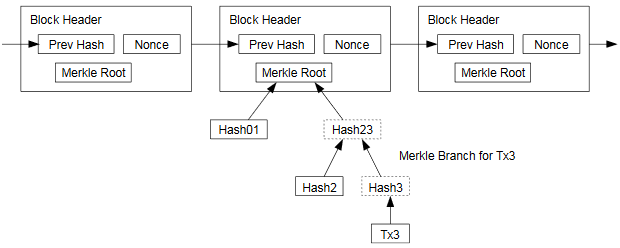
\includegraphics[width=\linewidth]{blockchain}
    \caption{Struttura di una blockchain.}
    \label{fig:blockchain}
\end{figure}

La \textbf{blockchain} è una architettura di calcolo distribuito funzionante come un registro elettronico senza intermediari
che garantisce l’immutabilità e la permanenza delle informazioni salvate su di essa.

Come suggerisce il nome, la blockchain è una catena di blocchi marcati temporalmente sempre crescente,
nella quale ogni blocco contiene queste informazioni:

\begin{itemize}
    \item Un insieme di transazioni salvate in un Merkle Tree (un albero binario crittograficamente verificato)
    \item L'hash del blocco precedente (nel caso di Ethereum e Bitcoin viene utilizzato l'algoritmo di hashing SHA-256)
    \item Il momento in cui il blocco è stato aggiunto alla catena (sottoforma di timestamp UNIX)
    \item Un nonce, ovvero un numero unico che, inserito in una funzione di hash assieme al resto delle informazioni del blocco,
    permette di ottenere un hash del blocco che è valido secondo dei requisiti (ad es. inizia con quattro zeri).
\end{itemize}

La sicurezza della blockchain è data dalle garanzie delle funzioni di hash: dato che l'header di ogni blocco contiene
l'hash del blocco precedente, se un qualsiasi blocco venisse modificato, il suo hash cambierebbe, e quindi invaliderebbe 
il collegamente al blocco successivo. Bisognerebbe quindi andare a ricalcolare l'hash di ogni blocco successivo,
ma data la dimensione attuale di una blockchain come Bitcoin e la difficoltà della rete
ciò sarebbe computazionalmente quasi impossibile.

La blockchain è nata con Bitcoin, sistema peer-to-peer per una valuta digitale creato da Satoshi Nakamoto nel 2009
basato su una blockchain distribuita e decentralizzata. 
Distribuzione e decentralizzazione sono fondamentali perché rendono la blockchain di fatto incensurabile
e senza un unico point-of-failure. Chiunque può unirsi alla rete Bitcoin: è sufficiente eseguire un client Bitcoin che gestisce un wallet, ovvero
una chiave privata, una chiave pubblica ed un indirizzo Bitcoin, e connette il dispositivo su cui è installato come nodo della rete.

Ethereum prende tutte le caratteristiche di Bitcoin e le amplia, a partire dalla criptovaluta nativa del sistema, l'Ether.
L'Ether, oltre a fungere da scambio di valore tra un utente della rete ed un altro, serve anche a pagare il gas, ovvero la tassa
introdotta per evitare lo spam di transazioni sulla rete, necessario per inviare transazioni che possono anche non avere valore,
ma possono ad esempio eseguire del codice.

Ethereum infatti rende la sua blockchain facilmente programmabile tramite \textbf{smart contract}, ovvero programmi scritti
in un linguaggio di programmazione ad alto livello come Solidity (simil-JavaScript) o Vyper (simil-Python),
compilati in bytecode e distribuiti sulla blockchain tramite transazioni. 
Gli smart contract sono eseguiti in un ambiente isolato ed indipendente (e quindi più sicuro)
chiamato \textbf{Smart Contract Execution Engine}, che nel caso di Ethereum prende il nome di EVM (Ethereum Virtual Machine).
Esattamente come in ogni blockchain distribuita e decentralizzata ogni nodo della rete possiede una copia della blockchain stessa
(e quindi ogni transazione), in Ethereum ogni nodo esegue il codice degli smart contract: questa replicazione rende molto lenta
l’esecuzione delle istruzioni, ma permette lo sviluppo di applicazioni che necessitano di trasparenza, sicurezza ed immutabilità.

\subsection{Perché Ethereum per BLINC?}
Nonostante la giovinezza del progetto, Ethereum si è già imposto come standard \emph{de-facto}
per lo sviluppo di applicazioni decentralizzate basate su smart contract
(è stato il primo a portare il concetto di smart contract su architetture
basate su blockchain, poi è stato seguito da altre architetture come Stellar e NEO)
e su un frontend che utilizza librerie come web3.js per comunicare con la rete Ethereum,
è supportato dalla più grande comunità open source in ambito blockchain ed è fornito di un grande numero
di strumenti per velocizzare il workflow di sviluppo di \emph{dApp} (Decentralized Applications), tra cui
Truffle, che facilita e automatizza task di compilazione e migrazione di contratti su diversi tipi di blockchain,
e Ganache, una simulazione in JavaScript di una blockchain locale che, in quanto non c'è bisogno di minare le
transazioni, è molto veloce e quindi adatta allo sviluppo e al testing di smart contract.

Essendo quindi un sistema stabile, ben supportato e facilmente integrabile con metodi di sviluppo tradizionali
grazie alle librerie in JavaScript costantemente aggiornate, Ethereum permette di rendere BLINC,
oltre che a un progetto di ricerca, un prodotto vendibile.

\section{Architettura generale del progetto}

\begin{figure}[!ht]
    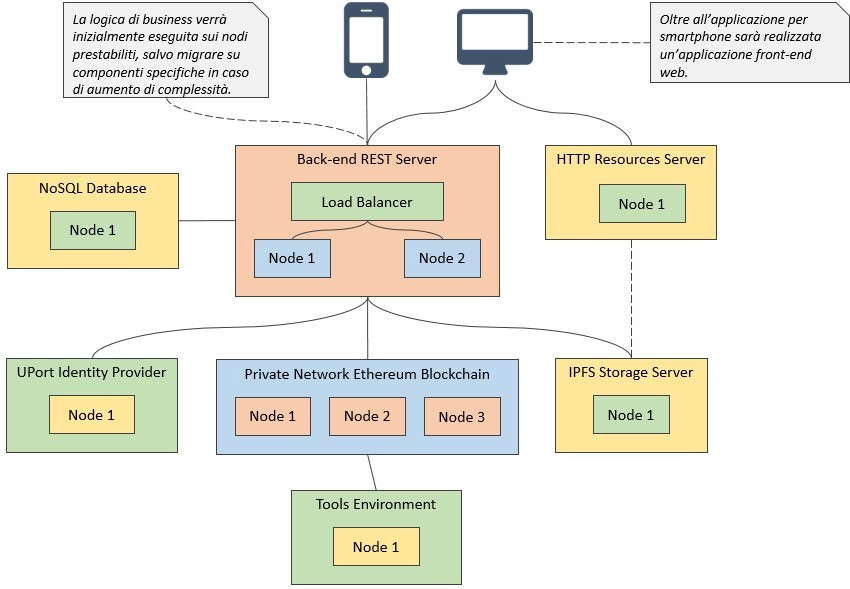
\includegraphics[width=\linewidth]{diagrammaarchitettura}
    \caption{Diagramma dell'architettura di BLINC.}
    \label{fig:diagrammaarchitettura}
\end{figure}

L’architettura è composta da (da sinistra a destra, dall’alto in basso):
\begin{itemize}
    \item Applicazione mobile (native Android ed iOS) e web app: servono ai migranti ed agli operatori per interfacciarsi ai servizi di BLINC.
    comunicano con i server REST e di risorse tramite chiamate ad API
    \item Database NoSQL (MongoDB): necessario per memorizzare informazioni e wallet criptati degli utenti
    \item Server di back-end (Loopback, framework di creazione di API basato su NodeJS): espone gli endpoint API richiamabili
    dai client, contiene la business logic e accede alla rete Ethereum per interagire
    con le identità dei migranti e effettuare dichiarazioni ed endorsement sulle generalità e documenti da essi caricati
    \item HTTP Resources Server: necessario per servire risorse statiche (immagini, documenti…) ai client
    \item uPort Identity Provider: insieme di \emph{smart contract} uPort distribuiti sui nodi Ethereum sottostanti che rendono
    possibile la creazione e gestione di identità e di attestazioni relative ad esse.
    \item Blockchain Privata Ethereum: insieme di nodi che eseguono istanze del client Ethereum Geth.
    \item IPFS Storage Server: un nodo IPFS, sistema di storage decentralizzato, necessario per salvare i documenti cifrati degli utenti.
    \item Tools environment: strumenti di monitoraggio della chain privata Ethereum citata in precedenza, in particolare un \emph{block explorer} ed un
    \emph{netstats}, che permettono rispettivamente di visualizzare le transazioni incluse per blocco e di avere una visione di insieme sulla rete Ethereum privata,
    tra cui la difficoltà della rete, i nodi che partecipano ad essa e l'uptime.
\end{itemize}

\subsection{Soluzione tecnologica}

\begin{figure}[!ht]
    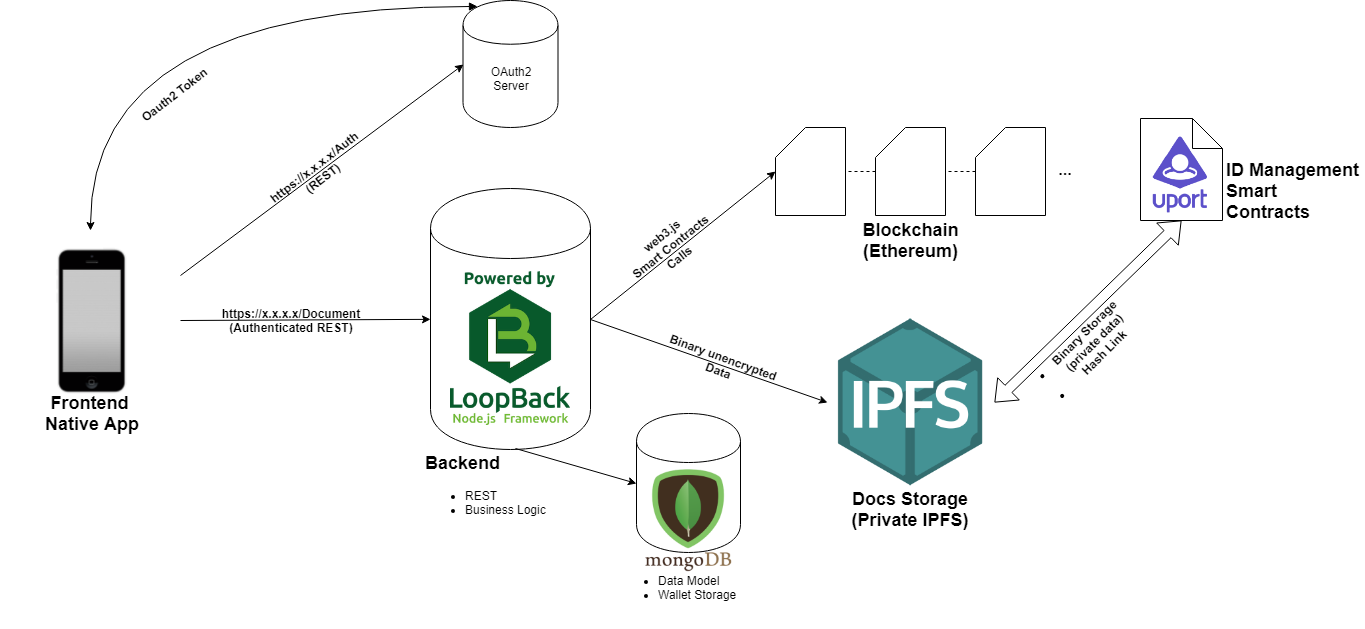
\includegraphics[width=\linewidth]{soluzionetecnologica}
    \caption{Soluzione tecnologica per BLINC.}
    \label{fig:soluzionetecnologica}
\end{figure}

Data l’immaturità del SDK di uPort che non ha permesso la creazione del wallet del migrante sul proprio telefono, la prima versione 
dell’architettura e di flusso di accesso ai servizi include elementi provvisori come l’OAuth server
(basato su login tramite e-mail e password e centralizzato, 
entrambe cose che si vorrebbero evitare) e il MongoDB (che contiene i wallet degli utenti criptati).	
In questa prima versione il flusso d’interazione base è quindi questo:

\subsubsection{Utente registrato}

L’utente apre l’applicazione di BLINC, inserisce e-mail/nome utente e password che vengono inviati all’OAuth server:
se e-mail/nome utente esistono e la password associata è corretta viene restituito un token di autorizzazione tramite il quale l’utente
potrà accedere alle API protette del backend.

Grazie al token ricevuto, l’utente può accedere innanzitutto alla propria identità uPort, salvata su database, 
per caricare documenti e verificare attestazioni sulle proprie credenziali e sui propri documenti.


\subsubsection{Utente non registrato}

Al primo accesso all’app BLINC il migrante inserisce informazioni base (nome, cognome, telefono…),
la propria e-mail ed una password. Queste ultime vengono salvate sull’OAuth server per i login successivi, 
l’identità viene creata con le informazioni inserite in precedenza tramite le librerie apposite di uPort 
e salvata su MongoDB, dove viene anche creato, criptato e salvato il wallet Ethereum dell’utente,
composto da una coppia di chiavi ed un indirizzo Ethereum, ricavato dalla chiave pubblica.
